\documentclass{beamer}

\usepackage[utf8]{inputenc}
\usecolortheme{beaver}
\usepackage{caption}
\usepackage{subcaption}
\usepackage{mathtools}
\usepackage{todonotes}
\usepackage{amsmath}
\usepackage{bm}
\usepackage{listings}
\usepackage{ragged2e}
\usepackage{titlecaps}
\usepackage{fancyvrb}

\def\ci{\perp\!\!\!\!\!\perp}

\newtheorem{proposition}{Proposition}
\Addlcwords{for a is but and with of in as the etc on to if}

\setbeamertemplate{section in toc}{\inserttocsectionnumber.~\inserttocsection}
\usetheme{Boadilla}
\makeatletter
\setbeamertemplate{footline}{%
    \leavevmode%
    \hbox{%
        \begin{beamercolorbox}[wd=.3\paperwidth,ht=2.25ex,dp=1ex,center]{author in head/foot}%
            \usebeamerfont{author in head/foot}\insertshortauthor\expandafter\beamer@ifempty\expandafter{\beamer@shortinstitute}{}{~~(\insertshortinstitute)}
        \end{beamercolorbox}%
        \begin{beamercolorbox}[wd=.55\paperwidth,ht=2.25ex,dp=1ex,center]{title in head/foot}%
            \usebeamerfont{title in head/foot}\insertshorttitle
        \end{beamercolorbox}%
        \begin{beamercolorbox}[wd=.15\paperwidth,ht=2.25ex,dp=1ex,right]{date in head/foot}%
            \usebeamerfont{date in head/foot}\insertshortdate{}\hspace*{2em}
            \insertframenumber{} / \inserttotalframenumber\hspace*{2ex} 
        \end{beamercolorbox}}%
        \vskip0pt%
    }
\makeatother

\begin{document}

\title[]{Canonical Correlation Based Mixed Data Conditional Independence Testing: Emprirical Analysis}
\author{}
\date{}

\maketitle

\begin{frame}{Mixed Data CI Tests}
	\begin{enumerate}
		\item Mutual Information based test (MI-CG): Used as baseline; implemented in R package `bnlearn'
		\item Likelihood Ratio Test (MXM)
		\item Hotelling's $T^2$ test on mixed data residualization.
	\end{enumerate}
\end{frame}

\begin{frame}{Likelihood Ratio Test (MXM)}
\end{frame}

\begin{frame}{Hotelling's $ T^2 $ test}
Given two mixed data residual matrices, $ R_\mathbf{x} $ and $ R_\mathbf{y} $

$$ Q(\mathbf{x}, \mathbf{y}) = \frac{1}{n} \left( d \times \hat{\Sigma}_d \times d^T \right) $$


$$
d = (R_{\mathbb{I}(\mathbf{x}=1)} \cdot R_{(\mathbf{y}=1)}, \, \ldots \ ,
R_{\mathbb{I}(\mathbf{x}=C_x)} \cdot R_{(\mathbf{y}=C_y)} )
$$

$$ \hat{\Sigma}_d = cov(d) $$

Under null, $ Q $ is asymptotically $ \chi^2 (\mid R_\mathbf{x} \mid \times \mid R_\mathbf{y} \mid) $ distributed.

\end{frame}

\begin{frame}{Pillai's Trace}

$$ \textit{V}(R_\mathbf{x}, R_\mathbf{y}) = \sum_{\rho \in \bm{\rho}(R_\mathbf{x}, R_\mathbf{y})} \rho^2 $$

No exact asymptotic distribution, F-approximation is used.

\end{frame}

\begin{frame}{Simulating Mixed Data}
	Given a DAG, $ D $ we simulate the data as:
	\begin{enumerate}
		\item If $ Y $ is continuous, $ Y = B Pa_Y + \epsilon $
		\item If $ Y $ is categorical use multinomial regression, $ Y \sim \lambda(B Pa_Y + \epsilon) $, where $ \lambda(x) = \frac{e^x}{1+e^x} $.
		\item If $ Y $ is ordinal, using proportional odds model. $ Y \sim \lambda(A + B Pa_Y + \epsilon) $.
	\end{enumerate}
\end{frame}

\begin{frame}{Calibration: Data Generation}
	We use the following DAG:
\begin{center}
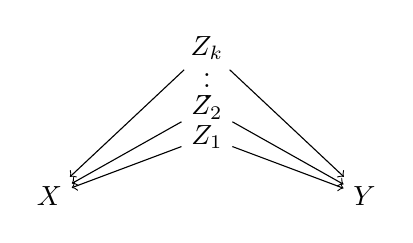
\begin{tikzpicture}[yscale=.75]
	\node (x) at (-1,1) {$X$};
	\node (y) at (3,1) {$Y$};
	\node (z) at (1,2) {$Z_1$};
	\node (z2) at (1, 2.5) {$Z_2$};
	\node (dots) at (1, 3) {$ \vdots $};
	\node (zk) at (1, 3.5) {$ Z_k $};
	\draw [->] (z) -- (y);
	\draw [->] (z) -- (x);
	\draw [->] (z2) -- (x);
	\draw [->] (z2) -- (y);
	\draw [->] (zk) -- (x);
	\draw [->] (zk) -- (y);
\end{tikzpicture}
\end{center}

\end{frame}

\begin{frame}{Calibration}
	\begin{figure}[t]
		\centering
		\includegraphics{conclusion.pdf}
		\caption{Calibration (left) and accuracy (right) comparison between the
		standard Hotelling's $ T^2 $ test, Adaptable Regularized Hotelling's $
		T^2 $ test (ARHT), Pillai-Bartlett Trace, and chi-squared test for CI
		testing in a low sample size and high cardinality scenario. Data has
		been simulated using the method outlined in
		Section~\ref{sec:emp_analysis} with both variables having $ 8 $
		categories each and $ 1 $ conditional variable. Sample size is $ 980 $
		which gives a ratio of $ 20:1 $ for number of samples to dimensionality
		for the $T^2$ tests.}
		\label{fig:conc_compare}
	\end{figure}
\end{frame}

\begin{frame}{Accuracy: Data Generation}
	We use the DAG:

\begin{center}
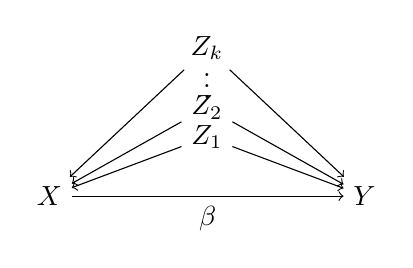
\begin{tikzpicture}[yscale=.75]
	\node (x) at (-1,0) {$X$};
	\node (y) at (3,0) {$Y$};
	\node (z) at (1,1) {$Z_1$};
	\node (z2) at (1, 1.5) {$Z_2$};
	\node  at (1, 2) {$ \vdots $};
	\node (zk) at (1, 2.5) {$Z_k$};
	\draw [->] (x) edge node [midway, below] {$\beta$} (y);
	\draw [->] (z) -- (y);
	\draw [->] (z) -- (x);
	\draw [->] (z2) -- (y);
	\draw [->] (z2) -- (x);
	\draw [->] (zk) -- (y);
	\draw [->] (zk) -- (x);
\end{tikzpicture}
\end{center}
\end{frame}

\begin{frame}{Accuracy}
	Insert figure here.
\end{frame}


\begin{frame}{Structure Learning: Data Generation}
	DAG generation mechanism.
\end{frame}

\begin{frame}{Structure Learning}
\end{frame}

\begin{frame}{Conclusion}
	\begin{itemize}
		\item Pillai's Trace is better calibrated especially in high-dimensional scenarios.
	\end{itemize}
\end{frame}

\end{document}
